\section{1174077 - Alvan Alvanzah}
\subsection{Soal Teori}
\begin{enumerate}

	\item Jelaskan dengan ilustrasi gambar sendiri apa itu generator dengan perumpamaan anda sebagai mahasiswa sebagai generatornya.
	\hfill\break
    Generator merupakan sebuah metode atau proses untuk menghasilkan data baru berdasarkan dengan data sebelumnya atau data yang ada. Biasanya output yang diminta haruslah sejenis sehingga misalkan dari Gambar seorang mahasiswa tidak bisa dijadikan output nilai dari mahasiswa yang berbentuk teks. Untuk generator sendiri, proses latihan bergantung pada seberapa sering input diterima dan perbandingan data yang asli dengan data yang dibuat oleh generator. Misalkan diberikan foto Mahasiswa 1 dijadikan patokan untuk output. Maka setiap input yang diterima akan dibandingkan dengan data yang sebenarnya. Semakin sering dilakukan generate atau pelatihan data, maka akurasi semakin tinggi.
    \hfill \break
    \begin{figure}[H]
	\centering
		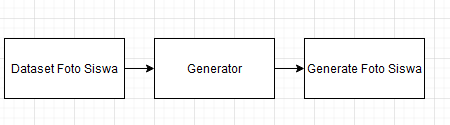
\includegraphics[width=4cm]{figures/1174077/8/t1.PNG}
		\caption{Ilustrasi generator}
	\end{figure}

	\item Jelaskan dengan ilustrasi gambar sendiri apa itu diskriminator dengan perumpamaan dosen anda sebagai diskriminatornya
    \hfill\break
    Discriminator merupakan pemisah antara data asli dengan data yang dihasilkan oleh generator. Discriminator akan menyimpan data yang ada ke kategori yang sudah didefinisikan sebelumnya. Discriminator sendiri akan membandingkan data input dengan pembanding sehingga dapat diketahui jika input itu adalah data palsu. Namun, jika terlalu sering dilakukan pelatihan generator maka discriminator sendiri akan berkurang akurasinya. Contohnya seperti misalkan Data dosen 1 dijadikan patokan dan input selalu dilakukan. Semakin sering dilatih, maka seseorang yang hampir mirip dengan dosen tersebut akan dapat diidentifikasikan sebagai data asli oleh discriminator.
    \begin{figure}[H]
	\centering
		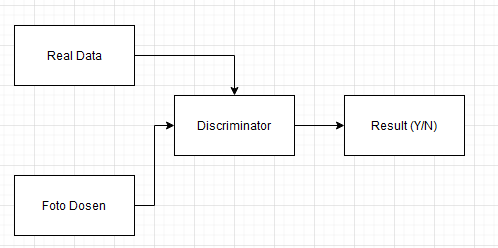
\includegraphics[width=4cm]{figures/1174077/8/t2.PNG}
		\caption{ilustrasi diskriminator}
	\end{figure}

	\item Jelaskan dengan ilustrasi gambar sendiri bagaimana arsitektur generator dibuat
	\hfill\break
	Arsitektur generator yang ada terbentuk dengan neural network sederhana yang terdiri dari beberapa layer. Untuk layernya sendiri ada layer input untuk menerima data. alu Dense layer atau layer proses untuk melakukan proses yang ada. Dan layer reshape untuk membentuk kembali data yang sudah diproses. Jumlah dari layer proses sendiri tergantung dari spesifikasi data yang ada.
    \begin{figure}[H]
        \centering
            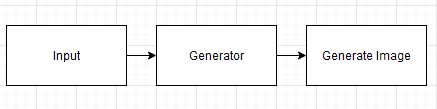
\includegraphics[width=4cm]{figures/1174077/8/t3.PNG}
            \caption{Ilustrasi pembuatan arsitektur generator}
        \end{figure}

	\item Jelaskan dengan ilustrasi gambar sendiri bagaimana arsitektur diskriminator dibuat
	\hfill\break
	Arsitektur Discriminator terdapat beberapa layer, diantaranya yaitu input layer untuk menerima data dari generator, output layer untuk mengindikasikan jika data yang diproduksi oleh generator yaitu asli atau tidak, dan layer proses untuk membandingkan data asli dengan data yang dihasilkan oleh generator.
    \begin{figure}[H]
	\centering
		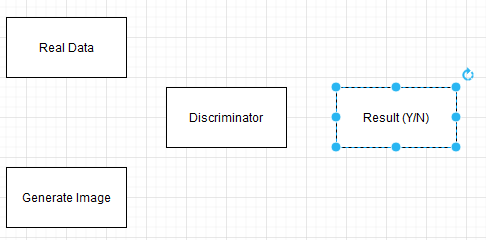
\includegraphics[width=4cm]{figures/1174077/8/t4.PNG}
		\caption{ilustrasi pembuatan arsitektur diskriminator}
	\end{figure}

	\item Jelaskan dengan ilustrasi gambar apa itu latent space.
	\hfill\break
	Latent space merupakan sebuah model yang menjabarkan isi dari data yang berbentuk media atau data yang tidak dikenali komputer, Seperti gambar, musik, dan lain sebagainya.
	\begin{figure}[H]
	\centering
		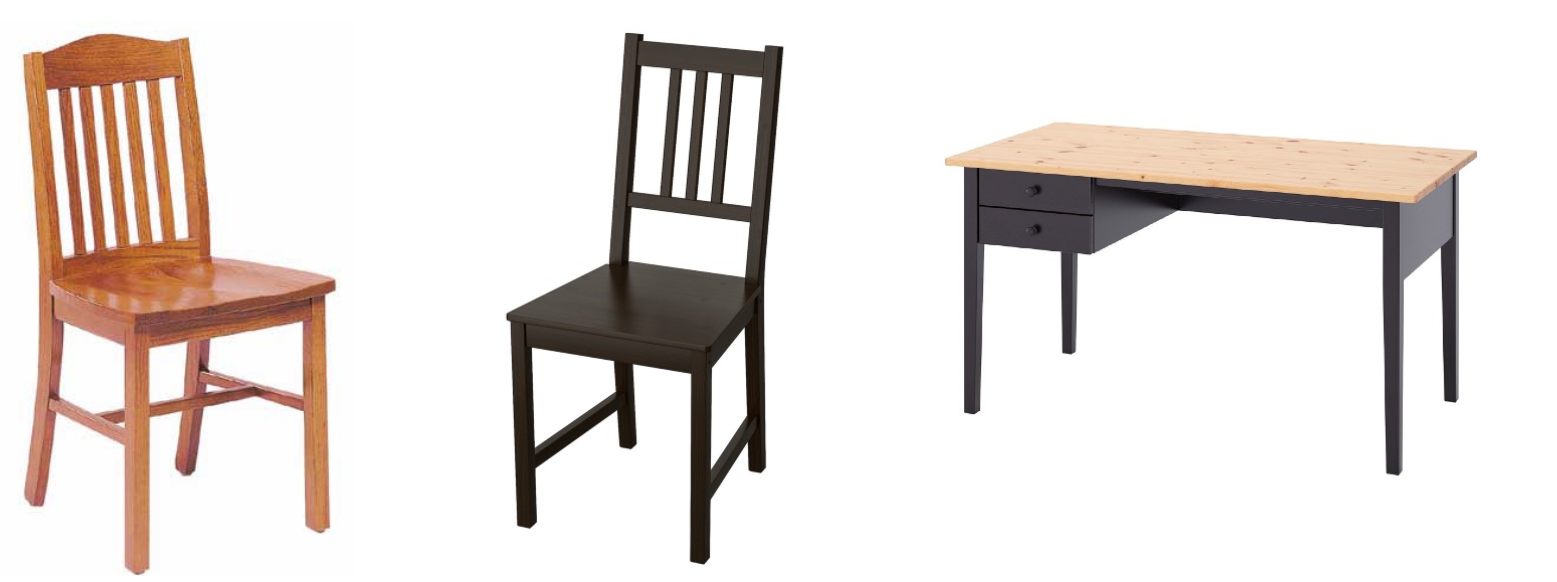
\includegraphics[width=4cm]{figures/1174077/8/t5.PNG}
		\caption{Ilustrasi latent space}
	\end{figure}

	\item Jelaskan dengan ilustrasi gambar apa itu adversarial play
	\hfill\break
	Adversarial play adalah dimana para jaringan di latih, dimana jaringan satu dan lainnya saling berkompetisi. dapat disimpulkan dimana jaringan generator dan jaringan discriminator saling bertemu berulang ulang kali.
	\begin{figure}[H]
	    \centering
	    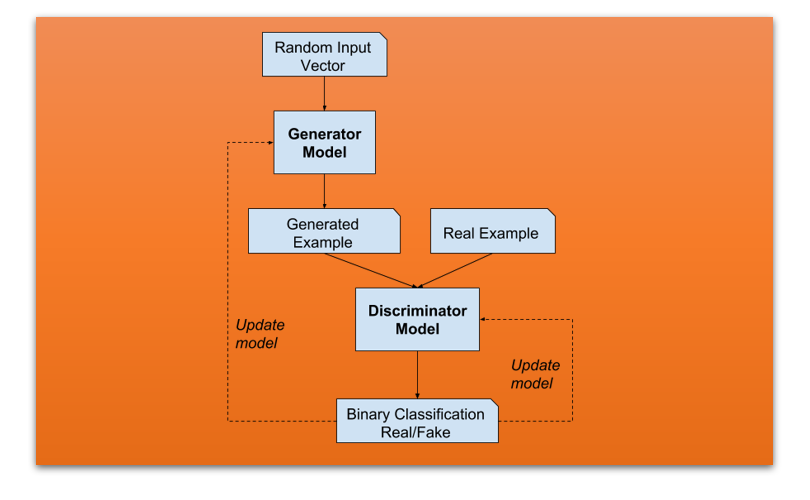
\includegraphics[width=4cm]{figures/1174077/8/t6.PNG}
	    \caption{Ilustrasi adversarial play}
    \end{figure}

    \item  Jelaskan dengan ilustrasi gambar apa itu Nash equilibrium
    \hfill\break
    Nash equilibrium adalah konsep dalam teori permainan di mana hasil optimal dari permainan adalah di mana tidak ada insentif untuk menyimpang dari strategi awal mereka. Lebih khusus lagi, keseimbangan Nash adalah konsep teori permainan di mana hasil optimal dari permainan adalah di mana tidak ada pemain yang memiliki insentif untuk menyimpang dari strategi yang dipilihnya setelah mempertimbangkan pilihan lawan.
    \begin{figure}[H]
	    \centering
	    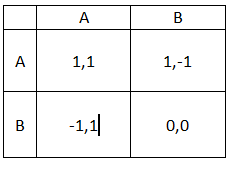
\includegraphics[width=4cm]{figures/1174077/8/t7.PNG}
	    \caption{ilustrasi nash equilibrium}
    \end{figure}

    \item Sebutkan dan jelaskan contoh-contoh implementasi dari GAN
    \hfill\break
    Pada bidang mode, seni, dan iklan, GAN dapat digunakan untuk membuat foto-foto model fashion imajinier tanpa perlu menyewa model. Pada bidang sains GAN dapat meningkatkan citra astronomi dan mensimulasikan pelensaan gravitasi untuk penelitian materi gelap.

    \item Berikan contoh dengan penjelasan kode program beserta gambar arsitektur untuk membuat generator(neural network) dengan sebuah input layer, tiga hidden layer(dense layer), dan satu output layer(reshape layer)
    \hfill\break
    \begin{verbatim}
        gen=Sequential() #Inisiasi dari sequensial
        gen.add(Dense(units=200,input_dim=np.shape(train_input)[1])) #Menambah dense layer dengan batch size 200 dan input dim dari input
        gen.add(Dense(units=400))#Menambah dense layer dengan batch size 400 dan input dim 100
        gen.add(Dense(units=784, activation='tanh')) #Menambah dense layer dengan batch size 784 dan aktivasi metode tanh
        gen.compile(loss='binary_crossentropy', optimizer=adam_optimizer()) #Menkompilasi hasil penambahan setiap dense
        gen.summary() #Memproses data yang sudah disetting dan menampilkannya
    \end{verbatim}
    \begin{figure}[H]
	    \centering
	    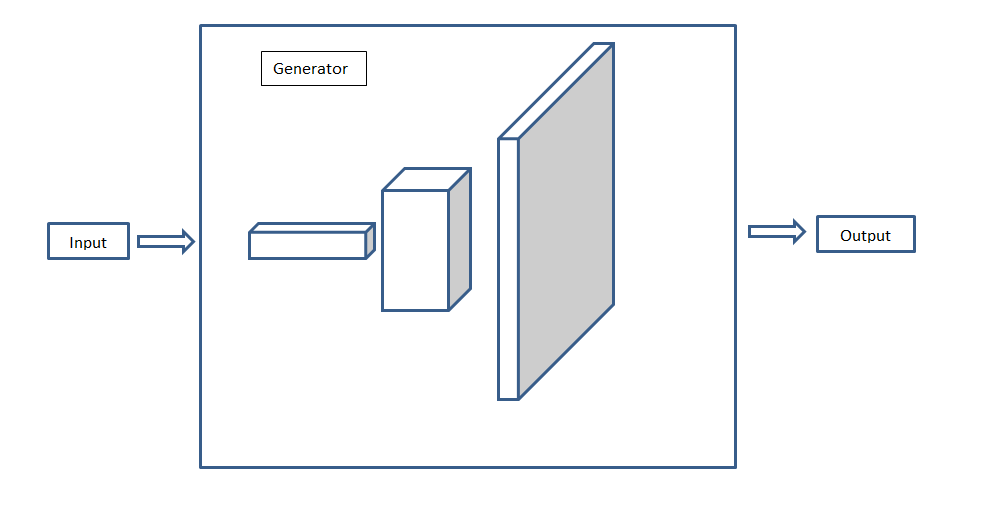
\includegraphics[width=4cm]{figures/1174077/8/t9.PNG}
	    \caption{arsitektur membuat generator}
    \end{figure}
    Pada contoh tersebut, data akan diambil dari hasil proses sebelumnya yaitu proses ekstrasi data gambar. Dari contoh ini, terdapat 3 layer dense, 1 input layer dan 1 output layer. Dari input layer nanti akan dimasukkan terlebih dahulu ke dense layer pertama lalu diproses oleh 2 layer selanjutnya dan terakhir akan ditampilkan oleh layer output.

    \item Berikan contoh dengan ilustrasi dari arsitektur diskriminator dengan sebuath input layer, 3 buah hidden layer, dan satu output layer.
    \hfill\break
    \begin{verbatim}
        diskrim=Sequential()#Inisiasi dari sequensial
        diskrim.add(Dense(units=784,input_dim=np.shape(train_input)[1]))#Menambah dense layer dan input dim dari layer
        diskrim.add(Dense(units=400)) #Mensetting Dense
        diskrim.add(Dense(units=200, activation='sigmoid')) #Mensetting dense dan melakukan aktivasi dengan metode sigmoid
        diskrim.compile(loss='binary_crossentropy', optimizer=adam_optimizer())#Menkompilasi hasil penambahan setiap dense
        diskrim.summary()#Memproses data yang sudah disetting dan menampilkannya
    \end{verbatim}
    Pada contoh tersebut, data akan diambil dari hasil proses sebelumnya yaitu proses ekstrasi data gambar. Dari contoh ini, terdapat 3 layer dense, 1 input layer dan 1 output layer. Pada proses ini, seluruh data akan dibandingkan dengan data sebelumnya yaitu dari generator dan dari data aslinya yang sudah dijadikan data vector. 
    \begin{figure}[H]
	    \centering
	    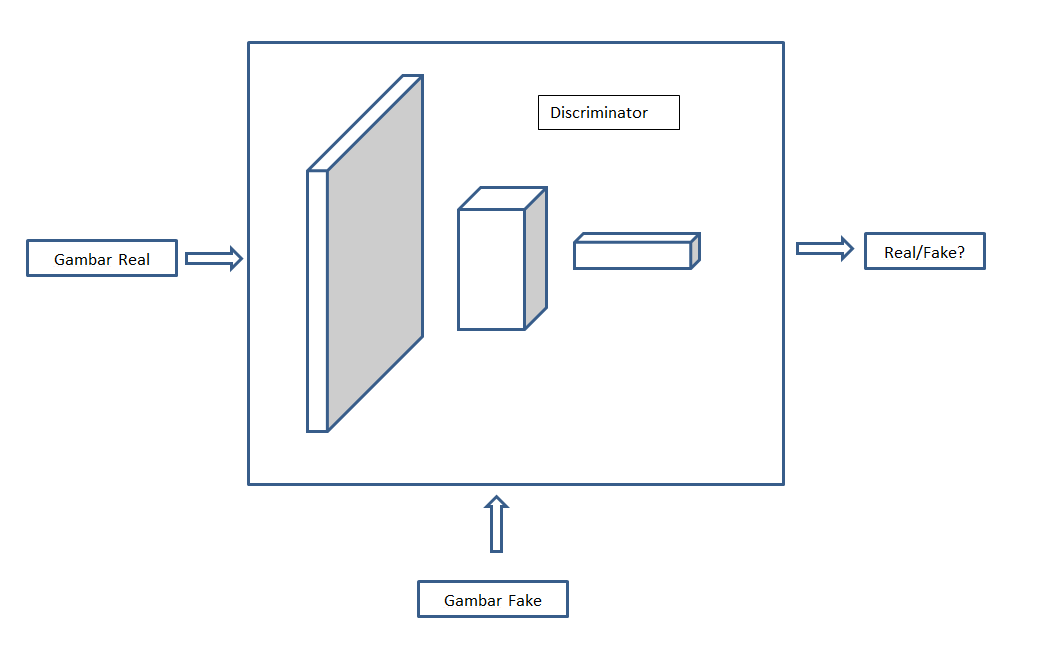
\includegraphics[width=4cm]{figures/1174077/8/t10.PNG}
	    \caption{arsitektur diskriminator}
    \end{figure}

    \item Jelaskan bagaimana kaitan output dan input antara generator dan diskriminator tersebut. Jelaskan kenapa inputan dan outputan seperti itu.
    \hfill\break
    Pada kedua metode tersebut, akan disebutkan berapa akurasi dari setiap metode. Pada setiap metode tersebut (Discriminator dan generator) akan dilakukan pelatihan dan akan dibandingkan hasilnya. Generator akan menghasilkan data baru sesuai dengan hasil latihan dan dari data tersebut, discriminator akan membandingkan dengan data set apakah data tersebut "asli" atau tidak. 

    \item Jelaskan apa perbedaan antara Kullback-Leibler divergence (KL divergence)/relative entropy, Jensen-Shannon(JS) divergence / information radius(iRaD) / total divergence to the average dalam mengukur kualitas dari model.
    \hfill\break
    Relative entropy adalah ukuran dari bagaimana satu distribusi probabilitas berbeda dari yang kedua, distribusi probabilitas referensi, Divergensi Jensen-Shannon adalah ukuran divergensi berprinsip yang selalu terbatas untuk variabel acak terbatas.
    
    \item Jelaskan apa itu fungsi objektif yang berfungsi untuk mengukur kesamaan antara gambar yang dibuat dengan yang asli.
    \hfill\break
    Fungsi objektif adalah fungsi yang digunakan sebagai penujuk berapa nilai kesamaan anatara gambar yang dibuat dengan yang asli.

    \item Jelaskan apa itu scoring algoritma selain mean square error atau cross entropy seperti The Inception Score dan The Frechet Inception distance.
    \hfill\break
    Inception Score digunakan untuk mengukur seberapa realistis output dari GAN, dimana ada dua parameter, yaitu : gambarnya punya variasi dan setiap gambar jelas terlihat seperti sesuatu. Frechet Inception Distance adalah ukuran kesamaan antara dua dataset gambar. Itu terbukti berkorelasi baik dengan penilaian manusia terhadap kualitas visual dan paling sering digunakan untuk mengevaluasi kualitas sampel Generative Adversarial Networks. FID dihitung dengan menghitung jarak Fr´echet antara dua Gaussians dipasang ke representasi fitur dari jaringan Inception.

    \item Jelaskan kelebihan dan kekurangan GAN
    \hfill\break
    \begin{itemize}
        \item GAN Menghasilkan data baru yang bisa hampir mirip dengan data asli. Karena hasil pelatihannya, GAN dapat menghasilkan data gambar, teks, audio, dan video yang dapat dibilang hampir mirip dengan yang aslinya. Berkat hal tersebut, GAN dapat digunakan dalam sistem marketing, e-commerce, games,iklan, dan industri lainnya
        \item GAN mempelajari representasi data secara internal sehingga beberapa masalah pada machine learning dapat diatasi dengan mudah
        \item Discriminator yang sudah dilatih dapat menjadi sebuah classifier atau pendeteksi jika data sudah sesuai. Karena Discriminator yang akan menjadi tidak efisien berkat seringnya dilatih
        \item GAN dapat dilatih menggunakan data yang belum dilabeled
    \end{itemize}
    Kerugian : \hfill \break
    \begin{itemize}
        \item Data saat diproses oleh metode gan tidak konvergensi
        \item Jenis sampel yang dihasilkan oleh generator terbatas karena modenya terbatas
        \item Ketidak seimbangnya antara generator dan discriminator dapat menyebabkan overfitting atau terlalu dekat dengan hasil sampel
        \item Sangat sensitif dengan data yang sudah diinisiasi sebelumnya
    \end{itemize}
\end{enumerate}

\subsection{Praktek Program}
\begin{enumerate}
	\item  Jelaskan apa itu 3D convolutions
    \hfill\break
    Konvolusi 3D menerapkan filter 3 dimensi ke kumpulan data dan filter 3 arah (x, y, z) untuk menghitung representasi fitur tingkat rendah. Bentuk outputnya adalah ruang volume 3 seperti kubus atau berbentuk kubus. 3D sangat membantu dalam pendeteksian peristiwa dalam video,gambarmedis 3D, dll. Generative Adversarial Network adalah arsitektur jaringan saraf tiruan yang dimaksudkan untuk membuat atau membuat data yang benar-benar baru, dari nol hingga tidak ada sama sekali. Melihat target utama GAN adalah data gambar. Singkatnya, jaringan GAN berfungsi untuk memberikan gambar baru berdasarkan koleksi gambar yang telah ada sebelumnya selama proses training. 
	
	\item  Jelaskan dengan kode program arsitektur dari generator networknya, beserta penjelasan input dan output dari generator network.
	\hfill\break
    \lstinputlisting[firstline=29, lastline=59]{src/1174077/8/run.py}
    Kode di atas akan melakukan create generator ialah gloss, Bentuk jaringan Generator dapat dilihat berkebalikan dengan struktur jaringan saraf pada umumnya. Generator biasanya menerima input sebuah vektor z, yang kemudian mengubahnya menjadi sebuah output 3D atau 3 dimensi.
    
	\item  Jelaskan dengan kode program arsitektur dari diskriminator network, beserta penjelasan input dan outputnya.
	\hfill\break
	\lstinputlisting[firstline=62, lastline=100]{src/1174077/8/run.py}
	Diskrimanator adalah d loss, Jaringan Diskriminator merupakan jaringan klasifikasi biner yang menerima input gambar tiga dimensi dan mengeluarkan klasifikasi menyatakan input gambar adalah gambar asli dari dataset atau merupakan gambar buatan Generator. Diskriminator dilatih dengan dataset yang diambil dari Generator, lalu di training untuk membedakan keduanya. Gambar dari Generator yang berhasil di deteksi oleh Diskriminator sebagai gambar fake, akan dikembalikan dengan feedback pke generator. Kini Generator bertugas untuk bisa membuat sekumpulan gambar palsu, yang nantinya dapat dilihat oleh Diskriminator, lalu, Diskriminator tidak bisa membedakan fake dan real.

	\item Jelaskan proses training 3D-GANs
    \hfill\break
    Proses training 3D GAN yaitu dengan melakukan epoch sebanyak yang ditentukan.

	\item Jelaskan bagaimana melakukan settingan awal chapter 02 untuk memenuhi semua kebutuhan sebelum melanjutkan ke tahapan persiapan data.
    \hfill\break
    \begin{itemize}
		\item Clone github
		\item Download dataset
		\item Buat folder baru logs dan results
	\end{itemize}

	\item Jelaskan tentang dataset yang digunakan, dari mulai tempat unduh, cara membuka dan melihat data. Sampai deskripsi dari isi dataset dengan detail penjelasan setiap folder/file yang membuat orang awam paham.
    \hfill\break
    Dataset yang digunakan yaitu 3DShapeNets yang berisi model model bentuk benda dll, folder train berisi train dan folder test berisi data testing. dan semua data tersebut di simpan didalam folder volumetric\_data.
	
	\item Jelaskan apa itu voxel dengan ilustrasi dan bahasa paling awam
    \hfill\break
    Volume pixel atau voxel adalah titik dalam ruang tiga dimensi. Sebuah voxel mendefinisikan posisi dengan tiga koordinat dalam arah x, y, dan z. Sebuah voxel adalah unit dasar untuk mewakili gambar 3D.

	\item Visualisasikan dataset tersebut dalam tampilan visual plot, jelaskan cara melakukan visualisasinya
    \hfill\break
    \lstinputlisting[firstline=281, lastline=301]{src/1174077/8/run.py}
    Kode di atas befungsi untuk visualisasidataset dalam tampilan plot. langkah-langkah seperti ini :
    import library, load data file .mat dan lakukan read memakai matplotlib, Hasilnya adalah sebagai berikut :
	\begin{figure}[H]
	\centering
		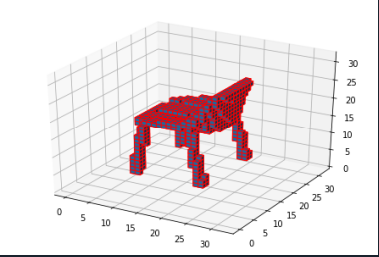
\includegraphics[width=4cm]{figures/1174077/8/p8.PNG}
		\caption{Hasil Soal 8.}
	\end{figure}

	\item buka file run.py jelaskan perbaris kode pada fungsi untuk membuat generator yaitu build generator.
	\hfill\break
	\lstinputlisting[firstline=29, lastline=59]{src/1174077/8/run.py}
	Kode di atas befungsi untuk membuat generator yaitu dengan ketentukan gen sebagai variabel dan membuat fungsi atau variabel genmodel lalu dilakukan return. 

	\item  jelaskan juga fungsi untuk membangun diskriminator pada fungsi build discriminator.
    \hfill\break
	\lstinputlisting[firstline=62, lastline=100]{src/1174077/8/run.py}
	Kode di atas befungsi untuk membangun diskriminator berfungsi untuk mendefenisikan seluruh gambar yang sudah di load generator sebagai gambar fake dan real.

	\item jelaskan apa maksud dari kode program name == ’ main ’
    \hfill\break
    Jika interpreter python menjalankan if name == main sebagai program utama, itu ialah menetapkan variabel name untuk memiliki nilai main. Jika file ini sedang di impor dari modul lain, name akan ditetapkan ke nama modul. Nama modul tersedia sebagai nilai untuk name variabel global.
    
    \item jelaskan secara detil perbaris dan per parameter apa arti dari kode program :
    \lstinputlisting[firstline=156, lastline=164]{src/1174077/8/run.py}
    \hfill\break
    Kode di atas befungsi untuk melakukan load dataset dengan ketentuan data yang hanya dalam folder chair pada data train.
        
    \item Jelaskan secara detil dari kode program pembuatan dan kompilasi arsitektur berikut :
    \lstinputlisting[firstline=170, lastline=177]{src/1174077/8/run.py}
    \hfill\break
    Kode di atas menggunakan Adam sebagai algoritma pengoptimalan dan binary\_crossentropy sebagai kerugian loss. 
    
    \item Jelaskan secara detil kode program untuk membuat dan melakukan kompilasi model adversarial berikut:
    \lstinputlisting[firstline=179, lastline=185]{src/1174077/8/run.py}
    \hfill\break
    Kode di atas artinya ialah kita memasukkan random vector kedalam generator model lalu membagi 2 yaitu generated example dan real example, dan meneruskan ke diskriminator model sebagai real atau fake
        
    \item Jelaskan Ekstrak dan load data kursi dengan menggunakan fungsi getVoxelsFormat dan get3DImages yang digunakan pada kode program berikut :
    \lstinputlisting[firstline=187, lastline=190]{src/1174077/8/run.py}
    \hfill\break
    Kode di atas befungsi untuk melakukan load data pada dataset.
        
    \item Jelaskan maksud dari kode program instansiasi TensorBoard yang menambahkan generator dan diskriminator pada program berikut: 
    \lstinputlisting[firstline=192, lastline=194]{src/1174077/8/run.py}
    \hfill\break
    Kode di atas berfungsi untuk membuat tensorboard yang nantinya bisa diakses melalui localhost.
    
    \item Jelaskan apa fungsi dari np reshape ones zeros pada kode program berikut dengan parameternya: 
    \lstinputlisting[firstline=196, lastline=197]{src/1174077/8/run.py}
    \hfill\break
    Kode di atas befungsi untuk melakukan reshape agar shape yang dihasilkan tidak terlalu besar. Dengan membuat variabel real dan fake.
        
    \item Jelaskan kenapa harus ada perulangan dalam meraih epoch. Dan jelaskan apa itu epoch terkait kode program berikut:
    \lstinputlisting[firstline=200, lastline=204]{src/1174077/8/run.py}
    \hfill\break
    Kode di atas befungsi untuk melakukan training epoch, karena jika epoch semakin banyak maka kualiatas training yang dihasilkan akan semakin baik.
        
    \item Jelaskan apa itu batches dan kaitannya dengan kode program berikut, dan kenapa berada di dalam epoch:
    \lstinputlisting[firstline=206, lastline=209]{src/1174077/8/run.py}
    \hfill\break
    Batch adalah jumlah file yang akan di training.
        
    \item Berikut adalah kode program pengambilan gambar dan noise. Jelaskan apa fungsi np.random.normal serta astype, serta jelaskan apa arti parameter titik dua dan jelaskan isi dari z sample dan volumes batch:
    \lstinputlisting[firstline=211, lastline=212]{src/1174077/8/run.py}
    \hfill\break
    Kode di atas befungsi untuk untuk membuat gambar bersih dari noise dan juga menyesuaikan shape.

    \item Berikut adalah kode program generator gambar palsu. Jelaskan apa fungsi generator.predict on batch, serta jelaskan apa arti parameter z sample:
    \lstinputlisting[firstline=214, lastline=215]{src/1174077/8/run.py}
    \hfill\break
    Kode di atas befungsi untuk membuat sample gambar palsu yang akan diteruskan ke diskriminator.

    \item Berikut adalah kode program training diskriminator dengan gambar palsu dari generator dan gambar asil. Jelaskan apa maksudnya harus dilakukan training diskriminator secara demikian dan jelaskan apa isi loss fake dan loss real serta d loss dan fungsi train on batch.
    \lstinputlisting[firstline=220, lastline=229]{src/1174077/8/run.py}
    \hfill\break
    Kode di atas befungsi untuk membuat diskriminator bisa load gambar fake dan real dari generator, oleh karena itu ada generator loss dan diskriminator loss untuk melihat seberapa baik kualitas yang dihasilkan.

    \item Berikut adalah kode program training model adversarial yang terdapat generator dan diskriminator. Jelaskan apa bagaimana proses terbentuknya parameter z dan g loss:
    \lstinputlisting[firstline=235, lastline=240]{src/1174077/8/run.py}
    \hfill\break
    Kode di atas befungsi untuk melakukan print gloss untuk generator dan juga dloss untuk diskriminator.

    \item  Berikut adalah kode program generate dan menyimpan gambar 3D setelah beberapa saat setiap epoch. Jelaskan mengapa ada perulangan dengan parameter tersebut, serta jelaskan arti setiap variabel beserta perlihatkan isinya dan artikan isinya :
    \lstinputlisting[firstline=242, lastline=250]{src/1174077/8/run.py}
    \hfill\break
    Mengapa ada perulangan ? karena untuk melakukan perbandingan dari hasil yang sudah didapat.

    \item Berikut adalah kode program menyimpan average losses setiap epoch. Jelaskan apa itu tensorboard dan setiap parameter yang digunakan pada kode program ini :
    \lstinputlisting[firstline=252, lastline=254]{src/1174077/8/run.py}
    \hfill\break
    TensorBoard adalah sebuah aplikasi web localhost untuk memeriksa dan menyelesaikan grafik dari hasil TensorFlow.
    
    \item Berikut adalah kode program menyimpan model. Jelaskan apa itu format h5 dan penjelasan dari kode program berikut :
    \lstinputlisting[firstline=259, lastline=260]{src/1174077/8/run.py}
    \hfill\break
    File H5 adalah file data yang disimpan dalam Format Data Hirarki (HDF). Ini berisi array multidimensi data ilmiah.

    \item Berikut adalah kode program testing model. Jelaskan dengan ilustrasi gambar dari mulai meload hingga membuat gambar 3D dengan menggunakan z sample, bisakah parameter z sample tersebut diubah2? :
    \lstinputlisting[firstline=263, lastline=279]{src/1174077/8/run.py}
    \hfill\break
    Ini adalah tahap akhir untuk melakukan testing dari model yang telah dibuat dan buat model dari yang sudah di create sebelumnya yaitu generator dan diskriminator. Untuk ilustrasi gambar sebagai berikut :
    \begin{figure}[H]
        \centering
            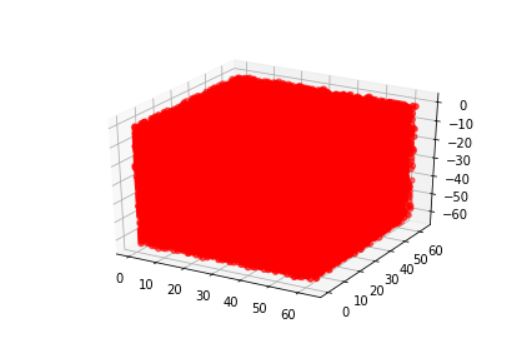
\includegraphics[width=4cm]{figures/1174077/8/p27.PNG}
            \caption{Hasil Soal 27.}
        \end{figure}
\end{enumerate}

\subsection{Penanganan Error}
\begin{enumerate}
	\item AttributeError: 'Model' object has no attribute 'get distribution strategy'
	\begin{figure}[H]
		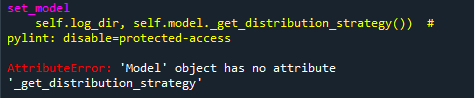
\includegraphics[width=4cm]{figures/1174077/8/error.PNG}
		\centering
		\caption{AttributeError}
	\end{figure}
	\item Tuliskan Kode Error dan Jenis Error
	\begin{itemize}
		\item AttributeError
	\end{itemize}
	\item Cara Penangan Error
	\begin{itemize}
		\item AttributeError
		\hfill\break
		Error terjadi karena versi tensorflow yang digunakan tidak sama dengan versi tensorflow yang disarankan oleh program sehingga tidak terdapat atribut untuk membangun model. Cara mengatasinya adalah dengan menginstall versi tensorflow yang sama dengan versi yang dibutuhkan oleh program. 
	\end{itemize}
\end{enumerate}

\subsection{Bukti Tidak Plagiat}
\begin{figure}[H]
\centering
	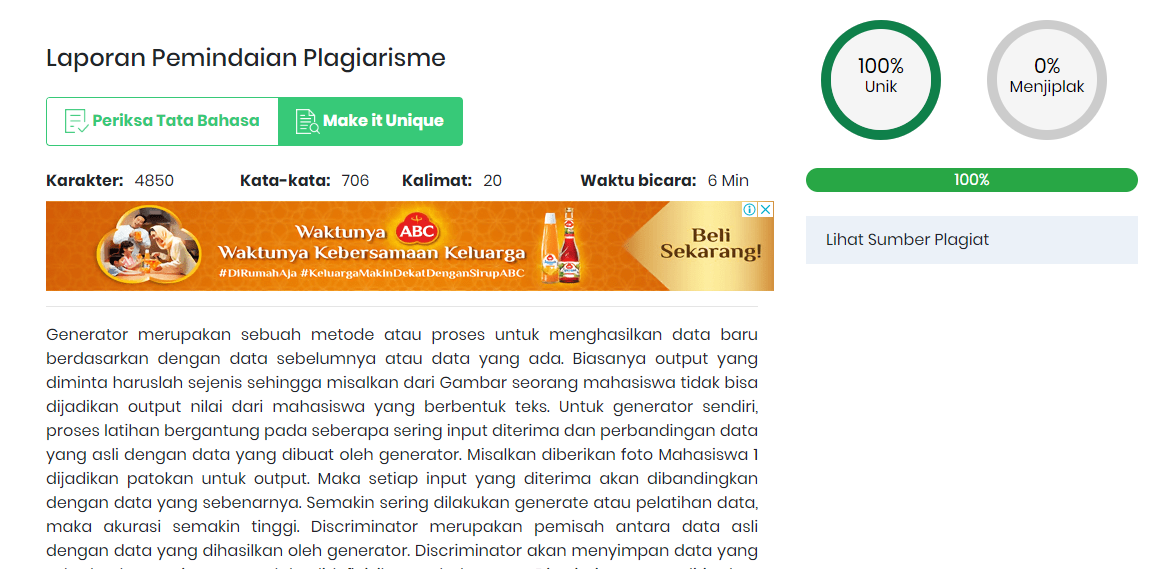
\includegraphics[width=4cm]{figures/1174077/8/plagiarisme.PNG}
	\caption{Bukti Tidak Melakukan Plagiat Chapter 8}
\end{figure}
